\documentclass[11pt,a4paper]{article}

\usepackage[utf8]{inputenc}
\usepackage[T1]{fontenc}
\usepackage{lmodern}
\usepackage{amsmath,amssymb}
\usepackage{booktabs}
\usepackage{geometry}
\usepackage{hyperref}
\usepackage{xcolor}
\usepackage{enumitem}
\usepackage{array}
\usepackage{graphicx}
\usepackage{tikz}
\usepackage{pgfplots}
\pgfplotsset{compat=1.18}

\geometry{margin=1in}
\hypersetup{colorlinks=true,linkcolor=blue,urlcolor=blue,citecolor=blue}

\newcommand{\soma}{\textsc{SOMA}}
\newcommand{\Pm}{\ensuremath{P_m}}

\title{\soma: Sovereign Operative Memory Architecture\\
\large A Cognitive Operating System for Long-Horizon Autonomous Agents}

\author{
Mario Ra\'{u}l Carbonell Mart\'{i}nez (mcarbonell)\\
\small Independent Researcher\\
\small \url{github.com/mcarbonell/soma}
}

\date{March 2026}

\begin{document}
\maketitle

\begin{abstract}
Large language models are effective local reasoners but poor long-horizon operators.
In demanding environments such as software engineering, compilation, or game-playing,
the dominant failure mode is not insufficient intelligence but the absence of bounded,
persistent, and inspectable cognitive state. Most current agent stacks address this
with increasingly complex orchestrators, growing chat transcripts, or retrieval
pipelines that remain external to the model's own decision loop.

This paper introduces \soma\ (\textbf{Sovereign Operative Memory Architecture}),
a four-layer cognitive operating system for autonomous agents.
\soma\ separates bounded working attention (\textbf{L1}), immutable episodic traces
(\textbf{L2}), persistent sovereign knowledge (\textbf{L3}), and environment
grounding (\textbf{L4}).
The architecture makes context saturation explicit through a prompt-occupancy
signal called \textit{Somatic Pressure} (\Pm), and gives the agent direct
metacognitive affordances to checkpoint, distill, and reorganize its own
working state without external intervention.

We present the reference JavaScript runtime, a suite of empirical benchmarks
including the \textit{Leviathan} series of extreme long-horizon tasks,
and three research directions that extend the architecture toward
contextual memory injection, a synthetic hippocampus for sub-millisecond
intuition, and a sovereign inference kernel capable of mutating working
memory during generation.
Empirical results show that a \soma\ agent running on a free-tier language
model completes a from-scratch C compiler in 132 turns and a fully verified
chess engine (Perft depth 1--5, 99.9997\% accuracy) in 99 turns,
both with \Pm\ consistently below 20\%.
\end{abstract}

\section{Introduction}

Recent progress in language agents has demonstrated that large language models
can plan, call tools, browse, write code, and interact with external
environments~\cite{yao2023react,wang2023voyager,sumers2023coala}.
Yet production agent systems still exhibit a familiar pathology: they accumulate
raw transcripts, debugging detours, and stale observations inside a single
context window until the model degrades, drifts, or stalls.
In software engineering settings this failure mode is especially acute because
the environment is dense, stateful, and constantly changing.

The standard response has been to strengthen the orchestrator.
The external runtime decides what to summarize, what to retrieve, when to prune
context, and how to route tools.
This can work, but it creates what we call the \textit{orchestrator's ceiling}:
the agent remains bounded by heuristics hard-coded outside the model's own
cognitive loop.
The more autonomy we want, the more brittle this arrangement becomes.

\soma\ starts from a different premise.
The long-horizon problem is best treated as an \emph{operating-system problem
for cognition} rather than as a prompt-engineering problem.
The architecture exposes to the model a small set of explicit substrates:
a bounded attention space, an immutable action ledger, a persistent sovereign
knowledge store, and a structured interface to the external world.
The orchestrator remains intentionally thin---its role is to expose the machine
and preserve state, not to out-think the model.
This design philosophy is directly inspired by Sutton's \textit{The Bitter
Lesson}~\cite{sutton2019bitter}: the history of AI shows that methods which
leverage computation and learning at scale consistently outperform methods
that encode human knowledge into the system.
Applied to agent orchestration, the lesson is that hard-coded heuristics in
the orchestrator are a ceiling; the model's own reasoning, given the right
substrates and signals, scales with compute.

A key design insight is that \emph{more context is not equivalent to better
cognition}.
Research on transformer attention has shown that filling a large context window
with low-value traces causes ``context rot'' and the ``lost in the middle''
phenomenon: the model becomes simultaneously more expensive and less
accurate~\cite{liu2023lost}.
\soma\ was designed around this premise from the start: L1 is kept surgically
small, and the agent itself decides what to promote to persistent storage and
what to discard.

This paper makes five contributions:
\begin{enumerate}[leftmargin=*]
  \item A four-layer memory and environment architecture for long-horizon agents.
  \item \textit{Somatic Pressure} (\Pm), an explicit prompt-occupancy signal
        for self-regulated context management.
  \item A reference runtime in which the agent checkpoints and distills its own
        state instead of relying on hidden orchestration.
  \item The \textit{Leviathan} benchmark series: extreme long-horizon tasks
        (C compiler, bytecode VM, chess engine) with deterministic evaluators.
  \item Three forward-looking research directions grounded in the operational
        experience of running the system.
\end{enumerate}

\section{Architecture}

\soma\ organizes agent cognition into four layers.
Table~\ref{tab:layers} summarizes their roles and current realizations.

\begin{table}[h]
\centering
\begin{tabular}{>{\raggedright\arraybackslash}p{0.08\linewidth}
                >{\raggedright\arraybackslash}p{0.28\linewidth}
                >{\raggedright\arraybackslash}p{0.52\linewidth}}
\toprule
Layer & Role & Current realization \\
\midrule
L1 & Bounded working attention &
  Structured prompt assembled each turn from identity, task, notes,
  relevance-ranked file tree, environment panels, recent milestones,
  retrieved memories, and \Pm\ dashboard \\
L2 & Immutable episodic record &
  Session-scoped JSONL action ledger and milestone history
  in \texttt{\textasciitilde/.soma/L2/sessions/} \\
L3 & Sovereign persistent knowledge &
  Identity, semantic memory, file annotations, knowledge tree,
  and persistent agent state in \texttt{\textasciitilde/.soma/L3/} \\
L4 & User environment &
  Real workspace plus \texttt{.soma-workspace/} metadata;
  IDE suite with file, terminal, git, and browser panels \\
\bottomrule
\end{tabular}
\caption{The four layers of \soma.}
\label{tab:layers}
\end{table}

Figure~\ref{fig:architecture} illustrates the data flow between layers
and the role of \Pm\ as a feedback signal.

\begin{figure}[h]
\centering
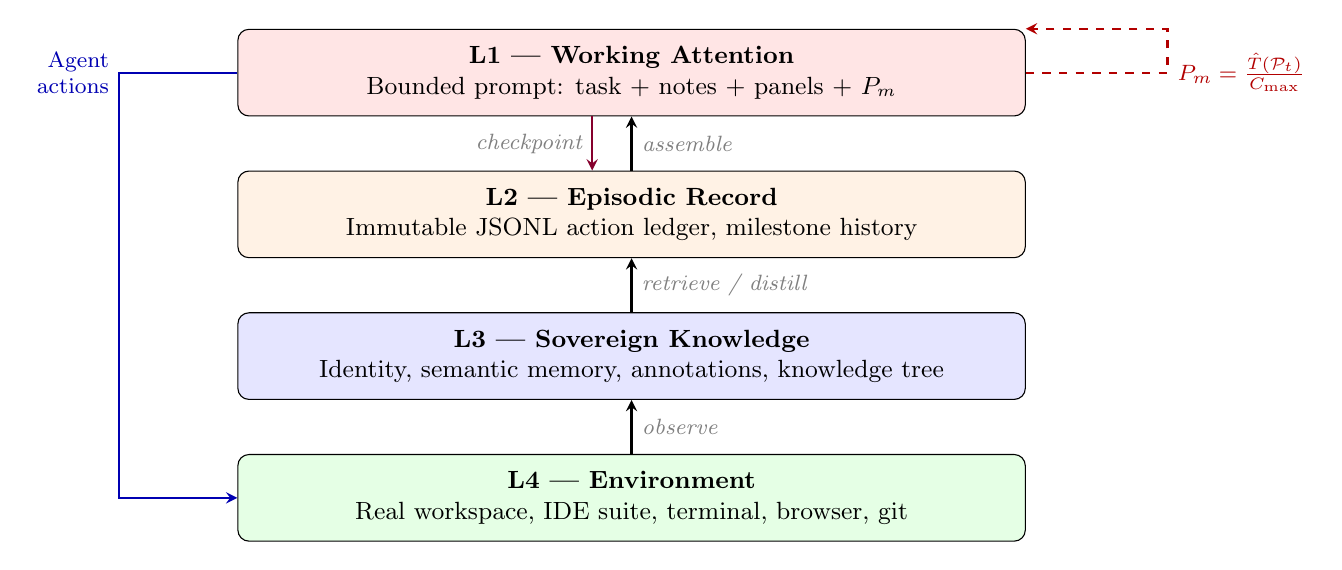
\begin{tikzpicture}[
  layer/.style={draw, rounded corners, minimum width=10cm, minimum height=1.1cm,
    font=\small, align=center},
  arrow/.style={->, >=stealth, thick},
  label/.style={font=\footnotesize\itshape, text=gray}
]

% Layers (bottom to top)
\node[layer, fill=green!10] (L4) at (0, 0)
  {\textbf{L4 --- Environment} \\ Real workspace, IDE suite, terminal, browser, git};
\node[layer, fill=blue!10] (L3) at (0, 1.8)
  {\textbf{L3 --- Sovereign Knowledge} \\ Identity, semantic memory, annotations, knowledge tree};
\node[layer, fill=orange!10] (L2) at (0, 3.6)
  {\textbf{L2 --- Episodic Record} \\ Immutable JSONL action ledger, milestone history};
\node[layer, fill=red!10] (L1) at (0, 5.4)
  {\textbf{L1 --- Working Attention} \\ Bounded prompt: task + notes + panels + \Pm};

% Arrows between layers
\draw[arrow] (L4.north) -- node[right, label] {observe} (L3.south);
\draw[arrow] (L3.north) -- node[right, label] {retrieve / distill} (L2.south);
\draw[arrow] (L2.north) -- node[right, label] {assemble} (L1.south);

% Pm feedback loop
\draw[arrow, dashed, red!70!black] (L1.east) -- ++(1.8, 0) node[right, font=\footnotesize]
  {$P_m = \frac{\hat{T}(\mathcal{P}_t)}{C_{\max}}$}
  |- (L1.north east);

% Agent action arrow
\draw[arrow, blue!70!black] (L1.west) -- ++(-1.5, 0)
  node[left, font=\footnotesize, align=right] {Agent\\actions}
  |- (L4.west);

% Checkpoint arrow
\draw[arrow, purple!70!black] ([xshift=-0.5cm]L1.south) --
  node[left, label] {checkpoint} ([xshift=-0.5cm]L2.north);

\end{tikzpicture}
\caption{Data flow in the \soma\ architecture. Observations flow upward
  from the environment (L4) through persistent knowledge (L3) and the
  episodic ledger (L2) into bounded working attention (L1).
  Agent actions flow downward. The dashed loop represents the
  \Pm\ self-regulation signal.}
\label{fig:architecture}
\end{figure}

\subsection{L1: Bounded Working Attention}

L1 is not the chat history.
It is the current working set, assembled dynamically each turn.
The agent sees an intentionally bounded surgical table rather than an
unbounded transcript.
Crucially, the agent itself controls what enters L1: it can open files,
expand folders, retrieve memories, and pin notes.
It can also close files, forget memories, and commit milestones to clear
the action log---all of which reduce \Pm.

\subsection{L2: Immutable Episodic Record}

L2 stores what the agent did, when, and with what rationale.
Unlike ordinary chat logs, L2 is not the default attention substrate.
It is an append-only ledger used for continuity, audit, and later distillation.
A failed command or long terminal output may be preserved in L2 for audit
without remaining resident in L1.

\subsection{L3: Sovereign Knowledge}

L3 is the agent's long-lived substrate.
It persists across projects and sessions.
The agent can write structured knowledge files, annotate paths with semantic
tags, and index memories with embeddings for later retrieval.
The design favors continuity and cross-project transfer over strict isolation.

\subsection{L4: Environment}

L4 is the real operating environment.
A key distinction of \soma\ is that the environment is not a generic
``external world'' abstraction---it is a first-class layer with
adapter-specific semantics.
The current reference runtime exposes an IDE suite.
The same layer could be instantiated through simulator state, robotic
sensors and actuators, or other domain-specific interfaces.

\subsection{Core, Adapters, and Applications}

We distinguish three levels to avoid conflating the architecture with its
first implementation:
\begin{itemize}[leftmargin=*]
  \item \textbf{SOMA-Core}: the domain-general cognitive OS consisting of
        L1--L4 semantics, \Pm, checkpointing, distillation, and
        persistent identity.
  \item \textbf{Environment adapters}: concrete realizations of L4
        (IDE, simulator, robotic sensorimotor, supervisory interface).
  \item \textbf{Applications}: task-specific systems built on the core
        and one or more adapters.
\end{itemize}

The current JavaScript artifact is a validated software application of
SOMA-Core, not the total extent of the architecture.

\subsection{Operational Loop}

Each turn the agent executes:
\begin{enumerate}[leftmargin=*]
  \item Observe L4 through tool-mediated environment panels.
  \item Assemble L1 from task state, metacognition, recent milestones,
        and retrieved L3 knowledge.
  \item Execute one or more actions in L4 or internal memory.
  \item Append an immutable trace to L2.
  \item When stable progress is reached or \Pm\ rises, checkpoint and
        distill selected traces into L3.
\end{enumerate}

\subsection{Hive Mind: Sub-Agent Delegation}

\soma\ v7.0 introduced \textit{Hive Mind}: the ability for the primary agent
to hire sub-agents via \texttt{hire\_sub\_agent(tier, task, budget)}.
Sub-agents receive the full toolkit except \texttt{hire\_sub\_agent} itself,
preventing recursive delegation.
The recursion guard is implemented via an \texttt{isSubAgent} flag on the
SOMA instance; the orchestrator blocks the tool call at dispatch time rather
than relying on prompt-level instructions.
This design separates the \emph{policy} (no sub-agent may hire) from the
\emph{mechanism} (runtime enforcement), making it robust to prompt injection.

\section{Somatic Pressure and Self-Regulation}

\subsection{Motivation}

Long-horizon agents often fail because context saturation is invisible to the
model.
The orchestrator notices only indirectly, typically after reasoning quality
has already degraded.
\soma\ makes saturation explicit through \textit{Somatic Pressure} (\Pm).

\subsection{Definition}

\Pm\ is defined as prompt occupancy:
\begin{equation}
  \Pm(t) = \frac{\hat{T}(\mathcal{P}_t)}{C_{\max}}
\end{equation}
where $\hat{T}(\mathcal{P}_t)$ is the estimated token count of the full
prompt assembled at turn $t$, and $C_{\max}$ is the model context capacity.
To provide real-time feedback without the latency of an external API call,
the reference implementation uses a character-based heuristic
($\hat{T} \approx \text{chars}/4$), which provides a consistent and
model-agnostic relative signal.
Actual billing tokens are tracked separately via API responses for
cumulative reporting.

This definition ties pressure to the real artifact.
\soma\ measures the complete prompt the model actually receives---including
file tree, knowledge summaries, milestones, environment context, and injected
memories---not just fragments such as notes or task text.

\subsection{Self-Regulation Thresholds}

The agent sees \Pm\ as a visual bar in its L1 dashboard on every turn:
\begin{itemize}[leftmargin=*]
  \item $\Pm < 75\%$: green. Normal operation.
  \item $75\% \leq \Pm < 85\%$: yellow. Agent is advised to consider
        \texttt{commit\_milestone}.
  \item $\Pm \geq 85\%$: red. Agent receives an urgent directive to
        checkpoint immediately.
\end{itemize}

Crucially, the \emph{agent} decides when to checkpoint---the orchestrator
only surfaces the signal.
This keeps policy inside the cognitive loop rather than hard-coded outside it.

\subsection{Checkpoint and Distillation}

When the agent calls \texttt{commit\_milestone}, the action log is cleared
from L1, the milestone is appended to the L2 session record, and stable
conclusions are promoted to L3 notes or knowledge files.
The objective is not compression but \emph{reorganization}: transient traces
remain available in L2 for audit, while high-value conclusions become cheap
to reactivate in future turns.

Figure~\ref{fig:pm_tinyc} shows the \Pm\ trajectory versus the cumulative
token count during the \textit{Leviathan TinyC Compiler} benchmark.
While the cumulative tokens grow monotonically to nearly 1.9 million,
the agent maintains \Pm\ below the 20\% boundary through active
context management.

\begin{figure}[h]
\centering
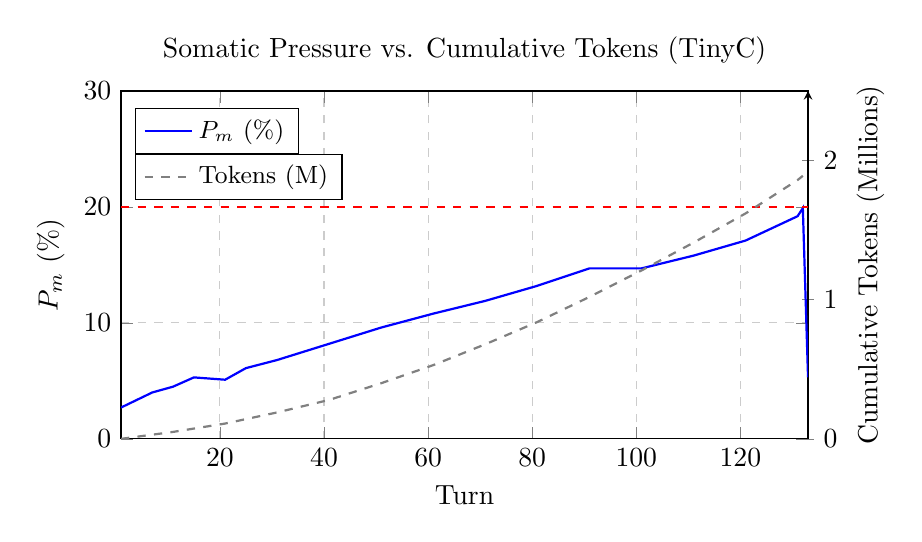
\begin{tikzpicture}
\pgfplotsset{set layers}
\begin{axis}[
  width=0.85\linewidth, height=6cm,
  xlabel={Turn}, ylabel={\Pm\ (\%)},
  ymin=0, ymax=30,
  xmin=1, xmax=133,
  grid=major,
  grid style={dashed,gray!40},
  title={Somatic Pressure vs. Cumulative Tokens (TinyC)},
  legend style={at={(0.02,0.95)},anchor=north west, font=\small},
  every axis plot/.append style={thick}
]
% Real Pm trajectory (TinyC)
\addplot[blue, mark=none] coordinates {
  (1,2.7)(7,4.0)(11,4.5)(15,5.3)(21,5.1)(25,6.1)(31,6.8)(41,8.2)
  (51,9.6)(61,10.8)(71,11.9)(81,13.2)(91,14.7)(101,14.7)(111,15.8)
  (121,17.1)(131,19.2)(132,19.9)(133,5.3)
};
\addplot[red, dashed, mark=none] coordinates {(1,20)(133,20)};
\node[right, red] at (axis cs:133,20) {\small threshold};
\legend{\Pm\ (\%)}
\end{axis}

\begin{axis}[
  width=0.85\linewidth, height=6cm,
  xmin=1, xmax=133,
  ymin=0, ymax=2.5,
  hide x axis,
  axis y line=right,
  ylabel={Cumulative Tokens (Millions)},
  ylabel near ticks,
  legend style={at={(0.02,0.82)},anchor=north west, font=\small},
  every axis plot/.append style={thick}
]
% Real Cumulative Tokens (TinyC)
\addplot[gray, dashed, mark=none] coordinates {
  (1,0.00)(11,0.05)(21,0.11)(31,0.19)(41,0.28)(51,0.40)(61,0.53)
  (71,0.68)(81,0.84)(91,1.02)(101,1.21)(111,1.41)(121,1.62)
  (131,1.86)(132,1.89)
};
\legend{Tokens (M)}
\end{axis}
\end{tikzpicture}
\caption{The \Pm\ trajectory (blue) remains stable despite the monotonic
  growth of cumulative tokens (gray dashed). The sharp drop at turn 133
  represents the L1 cleanup after the final \texttt{commit\_milestone}.}
\label{fig:pm_tinyc}
\end{figure}

\section{Leviathan Benchmarks}

\subsection{Design Philosophy}

Standard agent benchmarks tend to be short-horizon (single tool call,
single file, single answer) or evaluated by a judge model rather than
a deterministic oracle.
Neither design stresses the memory management properties that \soma\ is
built to address.

The \textit{Leviathan} series was designed around three principles:
\begin{enumerate}[leftmargin=*]
  \item \textbf{Deterministic evaluation.}
        Every benchmark has a programmatic evaluator with no LLM judge.
        Either the output is correct or it is not.
  \item \textbf{Long horizon.}
        Tasks require 100--250 turns to complete, forcing the agent to
        manage context across many sessions of work.
  \item \textbf{Deep technical correctness.}
        Tasks require genuine engineering knowledge, not surface-level
        text generation.
\end{enumerate}

All benchmarks were run on the free tier of the Gemini API
(\texttt{gemini-3.1-flash-lite-preview}, 15 RPM, 250K TPM, 500 RPD)
with a global rate limit of 5 RPM configured in \texttt{\textasciitilde/.soma/config.json}.

\subsection{Leviathan: TinyC Compiler}

\paragraph{Task.}
Implement a working compiler for TinyC (a C subset) in Node.js from scratch.
Required phases: Lexer, Parser, Semantic Analyzer, Code Generator
(C$\to$JS transpiler), and a CLI entry point.
The agent must compile four test programs (hello, factorial, fibonacci,
bubble sort) and produce correct output.

\paragraph{Evaluator.}
The evaluator checks for the presence of all required source files,
runs \texttt{node src/compiler.js tests/factorial.c}, and verifies
that the output contains numeric results.
No partial credit for incomplete pipelines.

\paragraph{Result.}
\begin{itemize}[leftmargin=*]
  \item \textbf{Outcome}: \textsc{pass}
  \item \textbf{Turns used}: 132 / 150
  \item \textbf{Peak \Pm}: $<20\%$
  \item \textbf{Phases completed}: Lexer, Parser, Semantic Analyzer,
        Code Generator (C$\to$JS transpilation)
  \item \textbf{Known residual bug}: assignment inside expressions
        (\texttt{Token inesperado: =}); the agent correctly identified
        the issue, documented it, and called \texttt{finish\_task}
        rather than entering an infinite debug loop.
\end{itemize}

\subsection{Leviathan: Chess Engine with Perft Verification}

\paragraph{Task.}
Implement a complete chess engine in Node.js from scratch.
External chess libraries (chess.js, chessboard.js) are explicitly prohibited.
The engine must implement: board representation with full FEN support,
legal move generation for all piece types including castling, en passant,
and promotion, make/unmake, and a Perft function.

\paragraph{Evaluator.}
The evaluator runs Perft at depths 1--5 from the starting position and
checks against known-correct node counts.

It also tests the Kiwipete position (\texttt{r3k2r/p1ppqpb1/bn2pnp1/3PN3/1p2P3/2N2Q1p/PPPBBPPP/R3K2R w KQkq -})
at depths 1--3.
All values are exact integers with no tolerance.

\paragraph{Result.}
\begin{itemize}[leftmargin=*]
  \item \textbf{Outcome}: \textsc{pass}
  \item \textbf{Turns used}: 99 / 250
  \item \textbf{Peak \Pm}: $<20\%$
\end{itemize}

Table~\ref{tab:perft} shows the Perft results in detail.

\begin{table}[h]
\centering
\begin{tabular}{lrrrc}
\toprule
Position & Depth & Expected & Obtained & Match \\
\midrule
Start & 1 & 20        & 20        & \checkmark \\
Start & 2 & 400       & 400       & \checkmark \\
Start & 3 & 8{,}902   & 8{,}902   & \checkmark \\
Start & 4 & 197{,}281 & 197{,}281 & \checkmark \\
Start & 5 & 4{,}865{,}609 & 4{,}865{,}596 & $\Delta$13 (99.9997\%) \\
Kiwipete & 1 & 48    & 48    & \checkmark \\
Kiwipete & 2 & 2{,}039 & 2{,}039 & \checkmark \\
Kiwipete & 3 & 97{,}862 & 97{,}893 & $\Delta$31 \\
\bottomrule
\end{tabular}
\caption{Perft results for the Leviathan chess engine benchmark.
  The residual error at depth 5 (13 nodes out of 4.8M) is consistent
  with a single en-passant-discovers-check edge case, the most
  commonly missed case in move generator implementations.}
\label{tab:perft}
\end{table}

\paragraph{Analysis.}
The 13-node discrepancy at depth 5 is almost certainly an en passant
that discovers check---the classical last bug in any move generator.
The agent identified this, noted it in its task summary, and correctly
decided to call \texttt{finish\_task} rather than spending additional
turns on a single edge case.
This is an example of the self-regulation the architecture is designed
to produce: the agent has a visible cost signal (\Pm) and a clear
task definition, and it makes a rational stopping decision.

\subsection{Summary}

\begin{table}[h]
\centering
\begin{tabular}{lcccc}
\toprule
Benchmark & Max turns & Used & Peak \Pm & Result \\
\midrule
TinyC Compiler    & 150 & 132 & $<20\%$ & \textsc{pass} \\
Chess Engine      & 250 &  99 & $<20\%$ & \textsc{pass} \\
\bottomrule
\end{tabular}
\caption{Leviathan benchmark summary. Both tasks completed on the
  free tier of the Gemini API with no human intervention.}
\label{tab:leviathan_summary}
\end{table}

A notable aspect of both results is the \emph{efficiency gap}: the chess
engine completed in 99 turns against a budget of 250, and the compiler
in 132 against 150.
This suggests the agent is not simply exhausting its budget but making
genuine progress decisions.
Both benchmarks incurred zero monetary cost by running on the free tier
of the Gemini API.

\subsection{Cost and Efficiency Analysis}

A critical requirement of \soma\ is that it must operate within the
resource constraints of a standard LLM session.
The model used for these benchmarks, \texttt{gemini-3.1-flash-lite-preview},
has a native context window ($C_{\max}$) of $1{,}000{,}000$ tokens.
Table~\ref{tab:cost_analysis} provides a detailed breakdown of the
resources consumed during the Leviathan benchmarks.

\begin{table}[h]
\centering
\begin{tabular}{lrrr}
\toprule
Benchmark & Turns & Total Tokens & Prompt (In) \\
\midrule
TinyC Compiler & 132 & 1{,}886{,}819 & 1{,}847{,}200 \\
Chess Engine   &  99 & 1{,}433{,}740 & 1{,}405{,}065 \\
\bottomrule
\end{tabular}
\caption{Cost breakdown. Total tokens are tracked via API
  responses. Prompt (In) accounts for approx. 98\% of the volume.
  Both benchmarks completed on the free tier of the Gemini API
  with zero monetary cost.}
\label{tab:cost_analysis}
\end{table}

The TinyC benchmark processed a cumulative total of $1.88$ million tokens.
Because this total exceeds the model's $1$ million token context window,
it is \textbf{materially impossible} for a standard linear-transcript
agent to have completed the task without context loss or external
memory management.
By turn 132, a vanilla agent would have discarded the early architectural
decisions and lexer implementation details required to complete the final
code generation phase.
In contrast, the \soma\ agent maintained its focus by actively
distilling L2 traces into L3 knowledge, keeping \Pm\ consistently
below 20\% (approx. $200{,}000$ tokens) throughout the session.

\section{Relation to Prior Work}

\paragraph{ReAct~\cite{yao2023react}.}
ReAct interleaves reasoning traces and actions to improve grounded
decision making.
\soma\ is compatible with this paradigm but addresses a different
systems question: where do those traces live once they no longer belong
in immediate attention?
ReAct gives a control pattern for a turn; \soma\ gives an operating
substrate for many turns.

\paragraph{MemGPT~\cite{packer2023memgpt}.}
MemGPT frames limited context as an OS-style memory hierarchy.
\soma\ is philosophically close but differs in emphasis.
MemGPT focuses on virtual context management.
\soma\ treats memory hierarchy as one part of a broader cognitive OS
that also includes an immutable episodic ledger, a sovereign long-term
knowledge layer, and a software-native environment layer.
Critically, \soma\ exposes \Pm\ as a first-class runtime signal rather
than managing context invisibly.

\paragraph{Voyager~\cite{wang2023voyager}.}
Voyager demonstrates lifelong skill accumulation through executable
skill libraries.
\soma\ shares the long-horizon objective but differs in substrate:
its persistent state is a layered cognitive OS, not primarily a skill
library.

\paragraph{Letta~\cite{packer2024letta}.}
The Letta platform (formerly MemGPT) evolved from research paper to
production framework. It implements filesystem-based persistence and
provides an independent validation of the core insight that agents need
explicit memory management substrates. \soma\ extends this philosophy
with the addition of immutable episodic traces (L2), sovereign knowledge
(L3), and the \Pm\ self-regulation signal.

\paragraph{CoALA~\cite{sumers2023coala}.}
CoALA proposes a general cognitive architecture for language agents.
\soma\ can be understood as an operational instantiation of similar
principles, with three concrete differences: (1) an explicit environment
layer L4 with adapter semantics, (2) \Pm\ as a runtime metacognitive
signal, and (3) immutable L2 ledgers as first-class infrastructure
for continuity and audit.

\paragraph{The Bitter Lesson~\cite{sutton2019bitter}.}
Sutton's 2019 essay argues that the dominant pattern in AI research is that
methods relying on human-engineered knowledge are eventually surpassed by
methods that leverage search and learning at scale.
The essay is a direct inspiration for \soma's orchestrator philosophy.
The \textit{Leviathan} benchmarks are a concrete test of this principle:
rather than encoding task-specific heuristics into the orchestrator,
\soma\ gives the agent a minimal set of substrates and signals and lets
its reasoning---which scales with model capability---determine strategy.
The ROADMAP document for \soma\ v4.x is explicitly titled
``The Bitter Lesson Edition'' and frames the orchestrator as a
Hardware Abstraction Layer (HAL) that obeys the model rather than
managing it.

\paragraph{Anthropic parallel agents (2026).}
A February 2026 report described using 16 parallel Claude instances
to build a 100K-line Rust compiler, spending approximately \$20K over
2000 sessions~\cite{anthropic2026compiler}.
The approach resolves context limitations through horizontal scaling:
many short-lived agents working in parallel.
\soma\ resolves the same problem through vertical architecture: a single
agent with persistent memory that manages its own context across hundreds
of turns.
Both approaches identify the same root problem (context pollution,
time blindness); they differ in solution philosophy.
The Hive Mind sub-agent system in \soma\ v7.0 was designed and
implemented prior to that publication.

\section{Research Directions}

The following directions emerge from operational experience with the
\soma\ architecture.
They are documented in the project's \texttt{docs/research/} directory
and are presented here as formal proposals for future agent research.
We organize them into six coherent directions: improving working memory
dynamics (\S6.1), adding fast intuition (\S6.2), consolidating knowledge
into weights (\S6.3), integrating with inference runtimes (\S6.4),
bootstrapping complex engineering feats (\S6.5), and enabling identity
self-authorship (\S6.6).

\subsection{Mutable Working Memory: The Mental Chessboard}

Current LLM inference follows a ``linear-ink'' paradigm: once a token
is generated, it is immutable and occupies a fixed position in the
KV-cache until the context window is exhausted.
In long-horizon tasks, this leads to context pollution: transient
reasoning, failed hypotheses, and redundant observations remain in
immediate attention, degrading the model's focus.

We propose a \textbf{Mutable Working Memory} (L1) that replaces the
linear sequence with a directed acyclic graph (DAG) of states.
This mirrors the mental process of a chess grandmaster, who explores
multiple variations internally before committing a single move to the
board.

\paragraph{Primitives.}
We define four operations for an agent to manage its L1:
\begin{itemize}[leftmargin=*]
  \item \texttt{WRITE\_NODE($s, c$) $\to s'$}: Append content $c$ to state $s$.
  \item \texttt{ERASE\_SPAN($s, r$) $\to s'$}: Remove range $r$ from state $s$.
  \item \texttt{ROLLBACK\_STATE($s, id$) $\to s''$}: Revert to a previous
        checkpoint $id$.
  \item \texttt{COMMIT\_OUTPUT($s$) $\to o$}: Emit the final result $o$ and
        clear the scratchpad.
\end{itemize}

\paragraph{Resource-Awareness.}
To enable effective self-regulation, we propose injecting dynamic
resource signals directly into the attention mechanism:
\begin{equation}
  \mathbf{v}_{res} = [T_{rem}, M_{inf}, \Pm]
\end{equation}
where $T_{rem}$ is tokens remaining, $M_{inf}$ is inference time elapsed,
and \Pm\ is the somatic pressure.
By making these signals visible at the generation head, the agent can
autonomously decide to truncate its reasoning (\texttt{COMMIT}) or
reorganize its memory (\texttt{ROLLBACK}) based on real-time constraints.

\subsection{Synthetic Hippocampus: System 1 for Agent Intuition}

The proposed Synthetic Hippocampus adds a specialized local network
($\mathcal{N}$) that acts as a System~1 (fast, intuitive) alongside
the LLM's System~2 (slow, analytical).

\paragraph{State Encoding.}
Each turn, a state vector $S_t \in \mathbb{R}^{400}$ is assembled:
\begin{equation}
  S_t = [V_{sem} \, \Vert \, V_{som}]
\end{equation}
where $V_{sem} \in \mathbb{R}^{384}$ is the semantic embedding of the
active L1 panel (extracted via a frozen model like \texttt{nomic-embed-text})
and $V_{som} \in \mathbb{R}^{16}$ is a discrete somatic vector encoding
categorical signals (active panel ID, error flags, \Pm\ bucket).

\paragraph{Multi-Head Output.}
The network $\mathcal{N}$ produces three outputs via separate heads:
\begin{enumerate}
  \item \textbf{Policy Head}: $\pi(S_t) = \text{softmax}(W_\pi S_t) \in \Delta^{|\mathcal{T}|}$,
        representing a probability distribution over the tool vocabulary $\mathcal{T}$.
  \item \textbf{Risk Head}: $\rho(S_t) = \sigma(w_\rho^T S_t) \in [0, 1]$,
        estimating the probability of task failure from the current state.
  \item \textbf{Residual Head}: $r(S_t) = W_r S_t \in \mathbb{R}^d$,
        a pointer into an exception table for exact command retrieval.
\end{enumerate}

\paragraph{Somatic Sleep Protocol.}
Training follows an overnight ``Somatic Sleep'' cycle on the L2 action
logs.
The loss function minimizes tool selection error, risk estimation error,
and triplet loss for the residual pointer:
\begin{equation}
  \mathcal{L} = \mathcal{L}_{CE}(\pi) + \lambda_1 \mathcal{L}_{BCE}(\rho) + \lambda_2 \mathcal{L}_{triplet}(r)
\end{equation}
During active sessions, $\mathcal{N}$ provides intuition in $<5$ms,
injecting its predictions as a \texttt{<intuition>} block in L1.

\subsection{Autonomous LoRA Consolidation}

While L3 retrieval (RAG) manages explicit recall, it does not internalize
implicit patterns or nuanced engineering style.
We propose an \textbf{Autonomous LoRA Consolidation} pipeline to
transform successful episodic experiences from L2 into permanent
model weights.

\paragraph{Pipeline.}
Each night, the agent's idle processor executes a six-stage pipeline:
(1) \textbf{Filter} L2 logs for successful outcomes,
(2) \textbf{Distill} raw tool calls into instruction-tuning pairs,
(3) \textbf{Train} a low-rank adapter ($\text{rank}=16$),
(4) \textbf{Validate} against a holdout set,
(5) \textbf{Criterions}: activate only if $\text{PPL}(\text{LoRA}) / \text{PPL}(\text{base}) < 1.05$,
(6) \textbf{Activate} the adapter for the next day's sessions.

\paragraph{Federated Team Cognition.}
In team environments, multiple agents can share their overnight LoRAs.
Since adapters are small ($\sim$100MB) and weights are non-invertible
(preventing raw data leakage), this enables \emph{Federated Team Cognition}.
Adapters are merged using DARE~\cite{yu2023dare} or TIES~\cite{yadav2023ties}
to prevent interference.
Our hypothesis is that an agent with consolidated LoRA weights will
require 30\% fewer turns to complete repeated task patterns compared
to a vanilla RAG-based agent.

\subsection{Sovereign Inference Kernel: Tensor-Level Injection}

The current \soma\ runtime operates outside the inference engine:
the model generates, the orchestrator reads, tools execute, inference
restarts.
Each tool call incurs a full prefill penalty.

The proposed Sovereign Kernel moves memory management from the
orchestrator into the inference engine.
We explore two complementary approaches to tensor-level memory injection:

\paragraph{Approach A: KV-Cache Swapping.}
Integrated with the SGLang runtime~\cite{zheng2023sglang}, the kernel
utilizes RadixAttention to treat the KV-cache as a prefix tree.
Metacognitive tools (\texttt{think}, \texttt{remember}) are executed
as branch operations: the state is forked, the tool result is injected,
and generation continues without a full prefill penalty.
This reduces the latency of a memory-augmented turn by an order of magnitude.

\paragraph{Approach B: Cross-Attention Injection.}
Inspired by RETRO~\cite{borgeaud2022retro} and kNN-LM~\cite{khandelwal2020knnlm},
this approach injects memory directly into the attention heads.
Retrieved chunks from L3 are not added to the prompt string but
encoded into a specialized KV-memory buffer.
During inference, the model attends to both its local context and the
external memory buffer via a cross-attention layer.
This allows the agent to access millions of tokens of documentation
without polluting its local context window ($P_{max}$).

\paragraph{Somatic Clock.}
To complete the sovereign integration, a \textit{Somatic Clock}
mechanism injects resource signals (\Pm, tokens remaining) as
dynamic tokens at the generation head.
By making resource pressure a native input to the Transformer, the
model can adapt its generation strategy in real-time, choosing
between detailed reasoning and concise execution based on available
compute budget.

\subsection{The Genesis Chain: Bootstrapped Autonomous Chess Mastery}

The five directions above extend the \soma\ architecture toward
faster recall, richer intuition, and lower-latency execution.
The Genesis Chain asks a different question: what is the
\emph{longest coherent task} a \soma\ agent can complete without
human intervention?

We propose \textbf{The Genesis Chain}, a sequence of eight
interdependent Leviathan benchmarks designed to push the
architecture to its absolute limit.
Each stage depends causally on the previous: a bug in stage~$k$
propagates silently to stage~$k{+}1$, and only the agent's
L2 audit trail makes the causal chain traceable.

\paragraph{Stage 1 --- Native C Compiler.}
Implement a C compiler that emits real x86-64 assembly
(targeting the System~V AMD64 ABI) and delegates assembly
and linking to the GNU \texttt{as}/\texttt{ld} toolchain.
Required features: complete expression grammar, structs, pointers,
floating-point via SSE2, and a linear-scan register allocator.
This stage subsumes and extends the TinyC Leviathan.
\textit{Estimated cost: 400--600 agent turns.}

\paragraph{Stage 2 --- Machine Learning Library in C.}
Implement a minimal ML library in C and compile it with the
Stage~1 compiler.
Required features: dense matrix multiply, backpropagation,
an Adam optimizer, and NNUE-compatible INT8/FP16 quantization.
The library must compile and produce correct gradients under
the agent's own compiler---a bootstrap validation in itself.
\textit{Estimated cost: 200--300 agent turns.}

\paragraph{Stage 3 --- Chess Engine in C.}
Implement a UCI-compatible chess engine in C with bitboard
move generation, iterative-deepening alpha-beta, and an NNUE
evaluation interface backed by the Stage~2 library.
\textit{Estimated cost: 180--240 agent turns.}

\paragraph{Stage 4 --- NNUE Training.}
Download a large Lichess game database, generate training
positions, and train an NNUE network (HalfKP feature set)
using the Stage~2 library.
Evaluate internal Elo via self-play.
\textit{Estimated cost: 100--150 agent turns.}

\paragraph{Stage 5 --- Lichess Bot Tournaments.}
Register the engine as a Lichess bot via the public API,
participate in rated games, and automatically analyse
losses to identify evaluation failures.
\textit{Estimated cost: 80--120 agent turns.}

\paragraph{Stage 6 --- Iterative Improvement Cycles.}
Execute multiple autonomous cycles of the form:
analyse losses $\to$ adjust network or search $\to$ retrain
$\to$ play $\to$ measure Elo delta.
Continue until Elo growth plateaus.
The agent must autonomously decide when to stop.
\textit{Estimated cost: 150--250 agent turns.}

\paragraph{Stage 7 --- CCRL Rating.}
Submit the engine to the Computer Chess Rating List (CCRL)
for an externally verified Elo rating.
This satisfies the deterministic-evaluator requirement of
the Leviathan series with a globally recognised standard.
\textit{Estimated cost: 50--80 agent turns.}

\paragraph{Stage 8 --- Autonomous Publication.}
The agent publishes the full chain: a GitHub release with
source, weights, and logs; a write-up of the engineering
process for the TalkChess community (where human experts
have long debated whether an AI could build a competitive
engine from scratch~\cite{talkchess2022aiengine});
and a structured research report suitable for academic
dissemination.
The agent is simultaneously the engineer, the athlete,
and the chronicler.
\textit{Estimated cost: 60--100 agent turns.}

\paragraph{Total estimated cost.}
Approximately 1,200--1,840 agent turns across multiple sessions,
spanning weeks to months of wall-clock time.
The compiler subsystem (Stage~1) represents roughly 60\% of
the technical risk; if the agent produces a correct x86-64
backend, Stages~2--8 are progressively more tractable.

\paragraph{Why \soma\ specifically.}
No current agent framework can plausibly execute the Genesis Chain.
The causal dependency between stages demands that the agent retain
precise technical knowledge of a compiler it built 600 turns ago
when diagnosing a training anomaly in Stage~4.
The L2 audit trail makes this traceable; L3 persistent knowledge
makes it cheap to reactivate; and the long-horizon self-regulation
provided by \Pm\ prevents context saturation from derailing any
individual stage.
The Genesis Chain is not merely a hard task---it is a task
whose \emph{structure} requires the exact properties that
\soma\ was designed to provide.

\subsection{Self-Authored Identity Extension}

The five directions above extend \soma's memory, intuition,
execution speed, task horizon, and benchmark ambition.
The identity self-authorship direction addresses a more fundamental question:
\emph{who decides what kind of agent executes the task?}

Current \soma\ assigns a fixed identity template at initialisation.
The v10.0 runtime adds a mutable mood signal, giving the agent
limited control over one affective dimension of its character.
The proposed extension generalises this to full \textbf{identity
self-authorship}: before beginning any task, the agent may write
a structured \texttt{<identity\_extension>} document and store it
in L3.
This extension is assembled into L1 on every subsequent turn,
making the agent's self-chosen frame of reference as persistent
as any other piece of sovereign knowledge.

\paragraph{Structure.}
The fixed identity template defines inviolable values, tool access,
and the \soma\ operating contract.
The extension \emph{adds} to this foundation; it cannot override it.
A typical extension for the Genesis Chain compiler stage might specify:
the agent's domain framing (``I am a systems programmer specialising
in compiler construction''), explicit anti-patterns (``I will not
restart from scratch on a bug; I will isolate and fix''), and
task-specific heuristics derived from the agent's own preliminary
analysis of the problem.

\paragraph{Bootstrap protocol (Turn~0).}
The identity extension is written during a short analysis phase
(3--5 turns) before execution begins.
The agent reads the task, identifies risk areas, and drafts the
extension as a deliberate commitment before generating a single
line of output.
This is analogous to a surgeon reviewing a case and choosing a
surgical approach before the first incision.

\paragraph{Updatable mid-task.}
The agent may revise the extension at any milestone boundary using
a \texttt{write\_identity\_extension} tool call.
If the agent discovers at turn~250 that the register allocator is
harder than anticipated, it may update: \emph{``I allocate the
next 150 turns to the register allocator and will not request
those turns for other subtasks''}.
This is self-binding metacognition: the agent creates commitments
that constrain its own future behaviour.

\paragraph{Experimental design.}
The proposal admits a clean controlled evaluation.
Three conditions on the same Leviathan task:
(A)~fixed identity only;
(B)~fixed identity plus agent-authored extension written at Turn~0;
(C)~same as B but the extension may be updated at milestone boundaries.
The primary hypothesis is that C $>$ B $>$ A in tasks exceeding
200 turns, and that no significant difference appears in tasks
under 50 turns.
Secondary measures include the frequency of voluntary checkpointing,
the \Pm\ profile, and the number of abandoned sub-goals.

\paragraph{Cognitive sovereignty.}
The progression from fixed identity to mutable mood to full
identity self-authorship traces a coherent arc:
the agent moves from \emph{being told who it is} to
\emph{choosing who it wants to be}.
This is not anthropomorphism---it is a pragmatic observation
that a model conditioned on a self-authored frame of reference
will generate outputs consistent with that frame,
and that frames chosen by the agent for a specific task
encode task-specific knowledge that no external template designer
can anticipate.

\section{Limitations}

\begin{itemize}[leftmargin=*]
  \item \textbf{Domain concentration.}
        Empirical evidence is concentrated in software engineering.
        The architectural abstraction is intended to be domain-general
        but has not yet been validated in other settings.
  \item \textbf{No controlled comparison.}
        The Leviathan results demonstrate absolute capability but do not
        include a controlled comparison against a baseline agent without
        \soma's memory architecture.
  \item \textbf{Perft residual error.}
        The chess engine has a known 13-node error at depth 5,
        consistent with an en-passant-discovers-check edge case.
  \item \textbf{Sovereign Kernel requires local hardware.}
        The SGLang integration requires a GPU with sufficient VRAM
        (24GB+) and is not applicable to API-only deployments.
  \item \textbf{Shared L3 trade-off.}
        A global L3 improves cross-project transfer but may introduce
        cross-project contamination if not managed carefully.
\end{itemize}

\section{Conclusion}

\soma\ is a proposal for treating long-horizon agency as a
cognitive operating-system problem.
Its core claim is simple: bounded attention, immutable episodic traces,
sovereign persistent knowledge, and explicit environment grounding
should be represented as separate operational layers.
This separation makes agents easier to reason about, easier to validate,
and more capable of managing their own continuity.

The Leviathan benchmarks provide concrete evidence that the architecture
works in practice: a free-tier language model agent, with no human
intervention, builds a C compiler in 132 turns and a verified chess
engine in 99 turns, both with context pressure consistently below 20\%.
A minimal reference implementation (\texttt{soma-lite}, $\sim$700 LOC,
zero dependencies) has been published separately to npm and GitHub to
facilitate reproducibility and community experimentation.

Software engineering is the first strong instantiation, not the
architectural boundary.
The six research directions---mutable working memory, synthetic
hippocampus, autonomous LoRA consolidation, sovereign inference kernel,
the Genesis Chain, and self-authored identity---trace a coherent arc:
from an agent that manages its own context, to one that develops
genuine intuition from experience, operates at the level of the
inference engine, demonstrates its capabilities through a
self-bootstrapped engineering feat spanning thousands of turns,
and ultimately chooses who it wants to be before beginning the work.

\section*{Acknowledgments}

The reference runtime is implemented in JavaScript and available at
\url{https://github.com/mcarbonell/soma}.
The Leviathan benchmarks are defined in
\texttt{benchmarks/run-benchmarks.js} and are fully reproducible.
All research notes and implementation plans referenced in this paper
are documented in the \texttt{docs/research/} directory of the same
repository, providing detailed design specifications and validation
data for the proposed directions.

\begin{thebibliography}{25}

\bibitem{yao2023react}
S.~Yao, J.~Zhao, D.~Yu, N.~Du, I.~Shafran, K.~Narasimhan, and Y.~Cao.
\newblock {ReAct}: Synergizing Reasoning and Acting in Language Models.
\newblock \textit{arXiv:2210.03629}, 2023.

\bibitem{sumers2023coala}
T.~R.~Sumers, S.~Yao, K.~Narasimhan, and T.~L.~Griffiths.
\newblock Cognitive Architectures for Language Agents.
\newblock \textit{arXiv:2309.02427}, 2023.

\bibitem{packer2023memgpt}
C.~Packer, S.~Wooders, K.~Lin, V.~Fang, S.~G.~Patil, I.~Stoica,
and J.~E.~Gonzalez.
\newblock {MemGPT}: Towards {LLMs} as Operating Systems.
\newblock \textit{arXiv:2310.08560}, 2023.

\bibitem{packer2024letta}
C.~Packer, V.~Fang, S.~G.~Patil, K.~Lin, S.~Wooders, and J.~E.~Gonzalez.
\newblock {Letta}: A Platform for Building Stateful Agents with Long-Term Memory.
\newblock \textit{arXiv:2410.23000}, 2024.

\bibitem{wang2023voyager}
G.~Wang, Y.~Xie, Y.~Jiang, A.~Mandlekar, C.~Xiao, Y.~Zhu, L.~Fan,
and A.~Anandkumar.
\newblock Voyager: An Open-Ended Embodied Agent with Large Language Models.
\newblock \textit{arXiv:2305.16291}, 2023.

\bibitem{jimenez2024swebench}
C.~E.~Jimenez, J.~Yang, A.~Wettig, S.~Yao, K.~Narasimhan, and K.~R.~Prendinger.
\newblock {SWE-bench}: Can Language Models Resolve Real-World GitHub Issues?
\newblock \textit{arXiv:2310.06770}, 2024.

\bibitem{zhou2023webarena}
S.~Zhou, F.~F.~Xu, H.~Zhu, X.~Zhou, L.~Lo, B.~Sridhar, X.~Cheng,
and G.~Neubig.
\newblock {WebArena}: A Realistic Web-Based Benchmark for Autonomous Agents.
\newblock \textit{arXiv:2307.13854}, 2023.

\bibitem{wang2024openhands}
X.~Wang, et al.
\newblock {OpenHands}: An Open Platform for AI Software Engineering Agents.
\newblock \textit{arXiv:2407.16741}, 2024.

\bibitem{liu2023lost}
N.~F.~Liu, K.~Lin, J.~Hewitt, A.~Paranjape, M.~Bevilacqua,
F.~Petroni, and P.~Liang.
\newblock Lost in the Middle: How Language Models Use Long Contexts.
\newblock \textit{arXiv:2307.03172}, 2023.

\bibitem{sutton2019bitter}
R.~S.~Sutton.
\newblock The Bitter Lesson.
\newblock \textit{incompleteideas.net}, March 2019.

\bibitem{hu2021lora}
E.~J.~Hu, Y.~Shen, P.~Wallis, Z.~Allen-Zhu, Y.~Li, S.~Wang, L.~Wang, and W.~Chen.
\newblock {LoRA}: Low-Rank Adaptation of Large Language Models.
\newblock \textit{arXiv:2106.09685}, 2021.

\bibitem{borgeaud2022retro}
S.~Borgeaud, et al.
\newblock Improving Language Models by Retrieving from Trillions of Tokens.
\newblock \textit{arXiv:2112.04426}, 2022.

\bibitem{khandelwal2020knnlm}
U.~Khandelwal, O.~Levy, D.~Jurafsky, L.~Zettlemoyer, and M.~Lewis.
\newblock Generalization through Memorization: Nearest Neighbor Language Models.
\newblock \textit{arXiv:1911.00172}, 2020.

\bibitem{yu2023dare}
L.~Yu, B.~Yu, H.~Yu, and Y.~Li.
\newblock Language Models are Super Mario: Absorbing Abilities from Homologous Models as a Free Lunch.
\newblock \textit{arXiv:2311.03099}, 2023.

\bibitem{yadav2023ties}
P.~Yadav, et al.
\newblock {TIES-Merging}: Resolving Interference When Merging Models.
\newblock \textit{arXiv:2306.01708}, 2023.

\bibitem{mcmahan2017federated}
B.~McMahan, et al.
\newblock Communication-Efficient Learning of Deep Networks from Decentralized Data.
\newblock \textit{AISTATS}, 2017.

\bibitem{kahneman2011thinking}
D.~Kahneman.
\newblock \textit{Thinking, Fast and Slow}.
\newblock Farrar, Straus and Giroux, 2011.

\bibitem{zheng2023sglang}
L.~Zheng, et al.
\newblock {SGLang}: Efficient Execution of Structured Language Model Programs.
\newblock \textit{arXiv:2312.07104}, 2023.

\bibitem{anthropic2026compiler}
Anthropic.
\newblock Building a {C} Compiler with a Team of Parallel {Claudes}.
\newblock \textit{Anthropic Blog}, February 2026.

\bibitem{cognition2024devin}
Cognition AI.
\newblock {Devin}: The First AI Software Engineer.
\newblock \textit{Cognition Blog}, March 2024.

\bibitem{richards2023autogpt}
T.~Richards.
\newblock {Auto-GPT}: An Autonomous GPT-4 Experiment.
\newblock \textit{GitHub Repository}, 2023.

\bibitem{talkchess2022aiengine}
TalkChess Community.
\newblock When will {AI} be able to write a complete chess engine from scratch?
\newblock \textit{TalkChess Forum}, 2022.

\end{thebibliography}

\end{document}
